\documentclass[11pt,a4paper]{article}

% =====================================================
% Pacotes
% =====================================================
\usepackage[utf8]{inputenc}
\usepackage[T1]{fontenc}
\usepackage[main=portuguese, provide=*]{babel}
\usepackage[a4paper, margin=2.5cm]{geometry}
\usepackage{graphicx}
\usepackage{xcolor}
\usepackage{hyperref}
\usepackage{booktabs}
\usepackage{float}
\usepackage{tabularx}
\usepackage{array}
\usepackage{tikz}
\usetikzlibrary{positioning, shapes.geometric, arrows.meta, fit, backgrounds, calc}
\usepackage{listings}
\usepackage{enumitem}
\usepackage{fancyhdr}
\usepackage{titlesec}
\usepackage{caption}
\usepackage[protrusion=true,expansion=false]{microtype}

% =====================================================
% Cabeçalho / Rodapé
% =====================================================
\pagestyle{fancy}
\fancyhf{}
\fancyhead[L]{\small Spot-On — Relatório Técnico}
\fancyhead[R]{\small LES 2025/2026}
\fancyfoot[C]{\thepage}
\renewcommand{\headrulewidth}{0.4pt}

% =====================================================
% Hyperlinks
% =====================================================
\hypersetup{
    colorlinks=true,
    linkcolor=blue!50!black,
    urlcolor=blue!60!black,
    citecolor=blue!50!black,
    pdftitle={Spot-On - Relatorio Tecnico},
    pdfauthor={Equipa Spot-On}
}

% =====================================================
% Estilo de código
% =====================================================
\definecolor{codebg}{RGB}{248,248,248}
\definecolor{codekw}{RGB}{0,80,160}
\definecolor{codecomment}{RGB}{120,120,120}
\definecolor{codestring}{RGB}{160,80,0}
\lstset{
    backgroundcolor=\color{codebg},
    basicstyle=\ttfamily\small,
    keywordstyle=\color{codekw}\bfseries,
    commentstyle=\color{codecomment}\itshape,
    stringstyle=\color{codestring},
    breaklines=true,
    frame=single,
    framesep=5pt,
    rulecolor=\color{gray!40},
    showstringspaces=false,
    captionpos=b,
    columns=fullflexible,
    keepspaces=true,
    inputencoding=utf8,
    extendedchars=true,
    literate=
        {á}{{\'a}}1 {à}{{\`a}}1 {ã}{{\~a}}1 {â}{{\^a}}1
        {é}{{\'e}}1 {ê}{{\^e}}1 {í}{{\'i}}1 {ó}{{\'o}}1
        {ô}{{\^o}}1 {õ}{{\~o}}1 {ú}{{\'u}}1 {ç}{{\c{c}}}1
        {Á}{{\'A}}1 {À}{{\`A}}1 {Ã}{{\~A}}1 {Â}{{\^A}}1
        {É}{{\'E}}1 {Ê}{{\^E}}1 {Í}{{\'I}}1 {Ó}{{\'O}}1
        {Ô}{{\^O}}1 {Õ}{{\~O}}1 {Ú}{{\'U}}1 {Ç}{{\c{C}}}1,
}

% =====================================================
% Cores para diagramas
% =====================================================
\definecolor{cClient}{RGB}{220,235,250}
\definecolor{cApp}{RGB}{210,240,220}
\definecolor{cData}{RGB}{250,235,210}
\definecolor{cExt}{RGB}{240,220,235}
\definecolor{cBorder}{RGB}{80,80,80}

\titleformat{\section}{\Large\bfseries\color{black!85}}{\thesection}{1em}{}
\titleformat{\subsection}{\large\bfseries\color{black!75}}{\thesubsection}{1em}{}

\begin{document}

% =====================================================
% Página de Rosto
% =====================================================
\begin{titlepage}
    \centering
    \vspace*{1.5cm}

    {\large Universidade do Algarve \par}
    {\normalsize Faculdade de Ciências e Tecnologia \par}

    \vspace{1cm}
    \rule{\linewidth}{0.4pt}\\[0.4em]
    {\Large\bfseries Laboratório de Engenharia de Software \par}
    {\normalsize Ano letivo 2025/2026 \par}
    \rule{\linewidth}{0.4pt}

    \vspace{3cm}

    {\Huge\bfseries Spot-On \par}
    \vspace{0.6cm}
    {\Large\itshape Sistema de Gestão de Espaços de Estudo \par}

    \vspace{2.5cm}

    {\large Relatório Técnico do Trabalho Prático \par}

    \vspace{2cm}

    \begin{tabular}{rl}
        \textbf{Docentes:} & Prof. José Barateiro \\
                           & Prof. Marco Giunti   \\
    \end{tabular}

    \vspace{1.5cm}

    \begin{tabular}{rl}
        \textbf{Equipa:} & André Martins -- n.º a35463  \\
                         & António Matoso -- n.º a84100 \\
                         & Tomás Machado -- n.º a84014  \\
                         & Vasco Hilário -- n.º 83993   \\
    \end{tabular}

    \vfill
    {\large \today \par}
\end{titlepage}

% =====================================================
% Índice
% =====================================================
\tableofcontents
\thispagestyle{fancy}
\newpage

% =====================================================
% 1. Introdução
% =====================================================
\section{Introdução}

O presente relatório documenta o trabalho prático desenvolvido no âmbito da
unidade curricular de Laboratório de Engenharia de Software, no ano letivo
2025/2026. O projeto, denominado \textbf{Spot-On}, consiste num sistema de
gestão de espaços de estudo, concebido para o contexto da biblioteca da
Universidade do Algarve.

A motivação para o tema surge de uma necessidade frequente entre estudantes:
identificar rapidamente que mesas individuais ou salas de grupo se encontram
disponíveis num determinado momento, sem percorrer fisicamente todos os pisos
da biblioteca. O Spot-On disponibiliza essa informação em tempo real através
de uma interface visual baseada nas plantas dos pisos, permitindo ainda
organizar sessões de estudo, convidar colegas, e gerir a ocupação dos espaços
com recurso a códigos QR.

Este documento descreve a visão geral do sistema, os atores envolvidos, os
requisitos funcionais e de qualidade, a arquitetura e o modelo de dados
adotados, bem como a justificação das principais decisões técnicas.

% =====================================================
% 2. Visão Geral do Sistema
% =====================================================
\section{Visão Geral do Sistema}\label{sec:overview}

O Spot-On é uma aplicação web que permite a alunos da Universidade do Algarve
visualizar e gerir o uso de espaços de estudo na biblioteca. O sistema
disponibiliza uma representação visual dos pisos da biblioteca, sobre a qual
são marcados os espaços (mesas individuais e salas de grupo), com indicação do
seu estado de ocupação em tempo real.

\subsection{Funcionalidades Principais}
\begin{itemize}[leftmargin=*]
    \item \textbf{Autenticação \emph{passwordless}} -- autenticação via
          \emph{magic link} enviado por email; o sistema permite restringir o
          acesso ao domínio institucional \texttt{@ualg.pt} através da variável
          de ambiente \texttt{ALLOWED\_EMAIL\_DOMAIN}, embora essa restrição
          esteja atualmente desativada na demonstração (ver \S5.4.3);
    \item \textbf{Visualização de plantas} -- exibição interativa das plantas
          dos pisos da biblioteca, com sobreposição dos espaços de estudo;
    \item \textbf{Gestão de espaços} -- mesas individuais e salas de grupo,
          com atributos como capacidade, presença de tomada elétrica, computador ou
          quadro interativo;
    \item \textbf{Sessões de estudo} -- criação, consulta e encerramento de
          sessões, associadas a um espaço e a um anfitrião (\emph{host});
    \item \textbf{Confirmação de presença via QR code} -- cada espaço dispõe
          de um \emph{token} QR rotativo que valida fisicamente a ocupação;
    \item \textbf{Convites e participações} -- o anfitrião pode convidar outros
          utilizadores para a sessão; estes confirmam ou rejeitam o convite;
    \item \textbf{Reports} -- mecanismo para reportar comportamentos
          incorretos, com confirmação por outros utilizadores e janela temporal
          limitada;
    \item \textbf{Notificações} -- sistema in-app para pedidos de adesão,
          pedidos de prova de presença e outros eventos relevantes;
    \item \textbf{Gamificação} -- atribuição automática de pontos e
          \emph{badges} (mensais, anuais ou permanentes) que premeiam a utilização
          regular e correta do sistema;
    \item \textbf{Administração (trabalho futuro)} -- o modelo de dados
          contempla já os campos necessários a moderação de utilizadores
          (e.g., \texttt{User.bannedUntil}) e gestão de \emph{badges}, mas a
          respetiva interface de administração não foi implementada na presente
          iteração.
\end{itemize}

\subsection{Levantamento Junto da Administração da Biblioteca}\label{sec:interview}

Para alicerçar a definição de requisitos numa visão real do problema, a
equipa realizou uma \textbf{reunião de levantamento com a administração da
Biblioteca da UAlg}. A reunião teve como objetivo perceber as queixas mais
frequentes recebidas pelos serviços, validar a viabilidade do conceito e
identificar limitações operacionais que o sistema deveria endereçar. A
tabela seguinte sumariza os principais pontos relatados e a forma como cada
um foi (ou não) endereçado pelo Spot-On.

\begin{table}[h!]
    \centering
    \footnotesize
    \renewcommand{\arraystretch}{1.35}
    \begin{tabularx}{\linewidth}{@{}>{\raggedright\arraybackslash}p{5.2cm}X@{}}
        \toprule
        \textbf{Relato da administração}                                                                                                                          & \textbf{Resposta do Spot-On}                                                                                                                                                                                                                                                                                                                                          \\
        \midrule
        Muitas queixas de \textbf{barulho} por parte dos alunos, com sugestão de mecanismos de advertência.                                                       & Implementado o sistema de \emph{Reports} entre pares (entidades \texttt{Report} e \texttt{ReportConfirmation}, com janela de 10~min para confirmação por terceiros), permitindo sinalização de comportamentos perturbadores sem necessidade de intervenção presencial do bibliotecário.                                                                              \\
        \midrule
        Estudantes que \textbf{deixam pertences (mochilas)} em mesas durante longos períodos sem as ocupar efetivamente --- prática contrária ao \emph{regulamento}. & Combinação de (i) sessão de estudo com \texttt{expectedEndTime} e expiração automática (\texttt{lib/session-expiry.ts}), (ii) \emph{Reports} de ocupação ilegítima por outros utilizadores e (iii) confirmação periódica de presença via QR code rotativo.                                                                                                          \\
        \midrule
        \textbf{Sistema de reservas} prévias é regularmente sugerido pelos alunos, mas a administração considera-o \emph{operacionalmente inviável} (sobrelotação fictícia, \emph{no-shows}). & A equipa alinhou-se com este \emph{feedback} e descartou o modelo de reserva antecipada. Optou-se por um modelo de \textbf{ocupação \emph{just-in-time}} com confirmação física via QR code no momento da chegada, eliminando \emph{no-shows} e garantindo que a planta reflete ocupação real.                                                                       \\
        \midrule
        \textbf{Aprovação geral} da ideia e da abordagem visual baseada em \textbf{plantas} dos pisos.                                                            & Validou a aposta na visualização gráfica (\texttt{FloorPlanSection}, \texttt{FloorPlanView}, \texttt{SpaceDetailPanel}) com polígonos SVG por espaço, suportando interação direta sobre a planta sem necessidade de identificadores textuais.                                                                                                                          \\
        \midrule
        Receio quanto à \textbf{veracidade da informação} em tempo real (e.g., utilizador sai sem terminar a sessão).                                             & Mitigação a três níveis: (i) QR \emph{token} rotativo (\texttt{currentQrToken} sincronizado por \texttt{node-cron}) que invalida fotografias antigas; (ii) pedidos de \emph{prova de presença} despoletados por \emph{Reports}; (iii) expiração automática da sessão ao atingir \texttt{expectedEndTime} ou o horário de fecho (\texttt{LIBRARY\_CLOSING\_TIME}). \\
        \midrule
        Nem todos os alunos têm \textbf{telemóveis} capazes de ler QR codes.                                                                                      & Limitação reconhecida. Está prevista como \textbf{trabalho futuro} a disponibilização de \emph{tablets} fixos junto a clusters de mesas (já contemplados em RQ-10) e/ou um fluxo alternativo de \emph{check-in} com código numérico curto.                                                                                                                            \\
        \midrule
        Sugestão de \textbf{desativar a aplicação em época de exames} para reduzir \emph{stress} dos estudantes.                                                  & \emph{Feedback} registado para discussão futura. A arquitetura permite, sem alterações de código, desligar funcionalidades sensíveis (e.g., \emph{Reports}) por configuração, viabilizando esta política se a administração assim o entender.                                                                                                                         \\
        \bottomrule
    \end{tabularx}
    \caption{Síntese da reunião com a administração da Biblioteca da UAlg e
        mapeamento para as funcionalidades do Spot-On.}
\end{table}

A reunião confirmou a pertinência do problema, validou as opções
arquiteturais centrais (visualização sobre plantas + QR code) e refinou o
âmbito do projeto (afastando o modelo de reserva antecipada). Os \emph{inputs}
recebidos são referenciados ao longo do relatório sempre que motivaram uma
decisão de \emph{design} concreta.

% =====================================================
% 3. Atores
% =====================================================
\section{Atores do Sistema}

O sistema tem um único ator humano implementado na presente iteração. Um
segundo ator (Administrador) está previsto como trabalho futuro --- o modelo
de dados já contempla a moderação (\texttt{User.bannedUntil}) e a configuração
de \emph{badges}, mas a respetiva interface de administração não foi
desenvolvida.

\begin{table}[h!]
    \centering
    \renewcommand{\arraystretch}{1.3}
    \begin{tabularx}{\linewidth}{@{}lX@{}}
        \toprule
        \textbf{Ator}                              & \textbf{Descrição}                                                                                                                                                                                                                                                            \\
        \midrule
        \textbf{Aluno}                             &
        Utilizador final do sistema. Pode autenticar-se, consultar a disponibilidade
        de espaços, criar e gerir sessões de estudo (anfitrião), participar em sessões
        de outros (convidado), submeter \emph{reports}, receber notificações e
        acumular pontos e \emph{badges}.                                                                                                                                                                                                                                                                                       \\
        \textbf{Administrador} \newline \emph{(trabalho futuro)} &
        Não implementado na presente iteração. Pretende-se, em fases futuras,
        disponibilizar uma interface de administração para gestão de plantas,
        espaços, \emph{badges} e moderação de utilizadores (banimento
        temporário, já suportado pelo modelo de dados).                                                                                                                                                                                                                                                                       \\
        \bottomrule
    \end{tabularx}
    \caption{Atores do sistema Spot-On.}
\end{table}

% =====================================================
% 4. Requisitos
% =====================================================
\section{Requisitos de Qualidade}\label{sec:req}

Os requisitos \emph{funcionais} do sistema encontram-se materializados como
\emph{user stories} no Jira, cada uma com critérios de aceitação claros e
ligada aos respetivos \emph{branches} e \emph{pull requests} no GitHub --- o
acesso ao \emph{board} foi partilhado com os docentes em modo de leitura.
Uma síntese funcional pode ainda ser consultada na descrição geral do
sistema (\S\ref{sec:overview}).

A presente secção foca-se nos requisitos \emph{de qualidade} (não
funcionais), que descrevem propriedades transversais ao sistema (segurança,
manutenibilidade, fiabilidade, etc.), tipicamente não capturadas em
\emph{user stories} individuais. A tabela seguinte enumera os requisitos
identificados, agrupados por categoria ISO/IEC~25010, com critérios
verificáveis sempre que possível.

\begin{table}[h!]
    \centering
    \footnotesize
    \renewcommand{\arraystretch}{1.3}
    \begin{tabularx}{\linewidth}{@{}llX@{}}
        \toprule
        \textbf{ID} & \textbf{Categoria} & \textbf{Descrição e Critério}     \\
        \midrule
        RQ-01       & Segurança          &
        O sistema dispõe de mecanismo de restrição de domínio de email
        (\texttt{ALLOWED\_EMAIL\_DOMAIN}), aplicado no \emph{backend} via
        \emph{callback} \texttt{signIn} do NextAuth. A restrição encontra-se
        atualmente desativada por motivos operacionais (ver \S5.4.3).        \\
        RQ-02       & Segurança          &
        Os \emph{tokens} de \emph{magic link} expiram em 5~minutos e só podem ser
        utilizados uma vez.                                                  \\
        RQ-03       & Segurança          &
        O \emph{token} QR de cada espaço é rotacionado periodicamente, impedindo a
        reutilização de fotografias antigas para validar presença.           \\
        RQ-04       & Segurança          &
        Utilizadores banidos (\texttt{bannedUntil} no futuro) não conseguem iniciar
        sessão nem participar em sessões.                                    \\
        RQ-05       & Manutenibilidade   &
        A camada de persistência é totalmente acedida através de um ORM, isolando o
        restante código de detalhes do SGBD.                                 \\
        RQ-06       & Manutenibilidade   &
        O \emph{schema} canónico em \texttt{prisma/schema.prisma} é a fonte
        única de verdade e está versionado em Git, com histórico de migrações
        em \texttt{prisma/migrations} geradas durante o desenvolvimento via
        \texttt{prisma migrate dev}. Em produção a base de dados é
        sincronizada com o \emph{schema} a cada \emph{deploy}.               \\
        RQ-07       & Portabilidade      &
        A aplicação executa em qualquer máquina com Docker instalado, através de um
        único comando (\texttt{docker compose up}), sem dependências locais
        adicionais.                                                          \\
        RQ-08       & Fiabilidade        &
        A \emph{pipeline} de CI executa, em cada \emph{push} e \emph{pull request},
        análise estática (\emph{lint}), testes automatizados e \emph{build} de
        produção; nenhum \emph{merge} em \texttt{main} ocorre sem que estes passos
        passem.                                                              \\
        RQ-09       & Usabilidade        &
        A consulta de disponibilidade é feita visualmente sobre a planta do piso,
        sem necessidade de o utilizador conhecer identificadores de espaços. \\
        RQ-10       & Compatibilidade    &
        A aplicação é responsiva e funciona em navegadores modernos (\emph{desktop} e
        \emph{mobile}), incluindo os tablets fixados nos espaços para exibir o QR
        code.                                                                \\
        \bottomrule
    \end{tabularx}
    \caption{Requisitos de qualidade do Spot-On.}
\end{table}

% =====================================================
% 5. Arquitetura e Stack Tecnológica
% =====================================================
\section{Arquitetura e Stack Tecnológica}\label{sec:arch}

A arquitetura do Spot-On foi desenhada com foco na \textbf{segurança},
\textbf{integridade dos dados} e \textbf{manutenibilidade}, utilizando uma
\emph{stack} moderna baseada em TypeScript. Esta secção descreve a visão de
alto nível, as camadas lógicas, a \emph{stack} adotada (com comparação a
alternativas, conforme exigido pelo enunciado) e as principais decisões
técnicas com as respetivas justificações.

\subsection{Visão de Alto Nível}

O Spot-On segue uma arquitetura \textbf{cliente-servidor} com aplicação web
\emph{full-stack} construída sobre Next.js. O \emph{frontend} (React) e o
\emph{backend} (API \emph{routes} do Next.js) coabitam no mesmo projeto, com
responsabilidades claramente separadas. A persistência é assegurada por uma
base de dados PostgreSQL, acedida exclusivamente através do ORM Prisma. A
autenticação é delegada à biblioteca NextAuth.js, que gere o fluxo de
\emph{magic link} com envio de email via Resend.

A Figura~\ref{fig:arch} apresenta o diagrama de componentes de alto nível do
Spot-On. O diagrama é mantido em formato \emph{drawio} no repositório
(\texttt{diagrams/component/backend\_arquitecture.drawio}) e exportado como
PNG para inclusão neste relatório. A análise das suas implicações
arquiteturais é discutida nas subsecções seguintes.

\begin{figure}[H]
    \centering
    % Substituir pelo PNG exportado do drawio quando estiver finalizado:
    % \includegraphics[width=0.9\linewidth]{figures/architecture_diagram.png}
    \vspace{1em}\textit{[Diagrama a inserir: \texttt{figures/architecture\_diagram.png}]}\vspace{1em}
    \caption{Diagrama de componentes de alto nível do Spot-On.}\label{fig:arch}
\end{figure}

\subsection{Camadas Lógicas}

Internamente, a aplicação Next.js encontra-se organizada em três camadas:

\begin{enumerate}[leftmargin=*]
    \item \textbf{Apresentação} -- componentes React responsáveis pela
          interface, incluindo a renderização das plantas, formulários e
          \emph{dashboards}. Faz uso de \emph{Server Components} e \emph{Client
              Components} consoante a necessidade de interatividade.
    \item \textbf{API e regras de negócio} -- \emph{API routes} do Next.js,
          onde reside a validação de dados, as regras de domínio (e.g.,
          elegibilidade para iniciar sessão, validade do QR \emph{token}, atribuição
          de pontos) e a orquestração das operações. Um \emph{middleware} global
          (\texttt{proxy.ts}) protege as rotas autenticadas, verificando a presença
          do \emph{cookie} de sessão NextAuth e redirecionando para a página de
          \emph{sign-in} quando ausente.
    \item \textbf{Persistência} -- camada de acesso a dados totalmente delegada
          ao Prisma, que gera um cliente tipado a partir do \emph{schema}
          \texttt{schema.prisma}.
\end{enumerate}

\subsection{Sumário da Stack e Alternativas}

A tabela seguinte resume, por camada, a tecnologia adotada (lado esquerdo) e
respetivamente a principal alternativa ponderada e a justificação resumida
(lado direito).

\begin{table}[H]
    \centering
    \footnotesize
    \renewcommand{\arraystretch}{1.35}
    \begin{tabularx}{\linewidth}{@{}>{\raggedright\arraybackslash}p{4.6cm}X@{}}
        \toprule
        \textbf{Camada \& Tecnologia adotada}                                                            & \textbf{Alternativa ponderada e justificação}                                                                                                          \\
        \midrule
        \emph{Framework} \emph{full-stack} \newline \textbf{Next.js (App Router, React)}                 & \textit{Alternativa:} React + Express separados. \newline
        \textit{Justificação:} unifica UI e API num único projeto, simplifica \emph{deployment} e permite tipagem partilhada entre cliente e servidor.   \\
        \midrule
        Linguagem (\emph{frontend} e \emph{backend}) \newline \textbf{TypeScript}                        & \textit{Alternativa:} JavaScript. \newline
        \textit{Justificação:} mesma linguagem em ambas as vertentes, com tipagem estática que reduz erros e integra-se com o cliente Prisma gerado.    \\
        \midrule
        ORM \newline \textbf{Prisma}                                                                     & \textit{Alternativa:} TypeORM, Sequelize. \newline
        \textit{Justificação:} \emph{schema} declarativo, migrações automáticas e tipagem forte ponta-a-ponta.                                          \\
        \midrule
        Base de dados \newline \textbf{PostgreSQL 17}                                                    & \textit{Alternativa:} MySQL, MongoDB. \newline
        \textit{Justificação:} modelo relacional adequado às entidades; \texttt{enum types} nativos; \emph{ACID compliance} e maturidade comprovada.    \\
        \midrule
        Autenticação \newline \textbf{NextAuth.js (\emph{magic link})}                                   & \textit{Alternativa:} Auth0, Clerk, implementação própria. \newline
        \textit{Justificação:} integração nativa com Next.js; fluxo \emph{passwordless} pronto a usar, sem armazenar \emph{passwords}.                  \\
        \midrule
        Envio de email \newline \textbf{Resend (API HTTP)}                                               & \textit{Alternativa inicial:} Nodemailer + SMTP. \newline
        \textit{Justificação:} adoção de API HTTP transacional, sem necessidade de servidor SMTP próprio; o Resend não disponibiliza \emph{endpoint} SMTP no \emph{free tier}, obrigando à migração do \emph{adapter} \texttt{nodemailer} para o cliente HTTP nativo. Ver \S5.4.6.                                                                                                                                       \\
        \midrule
        Containerização \newline \textbf{Docker + Docker Compose}                                        & \textit{Alternativa:} VM dedicada, \emph{deploy} direto na máquina. \newline
        \textit{Justificação:} \emph{setup} reprodutível em qualquer máquina com um único comando (\texttt{docker compose up}).                         \\
        \midrule
        Plataforma de \emph{deploy} \newline \textbf{Railway}                                            & \textit{Alternativa:} Vercel, Render, AWS Elastic Beanstalk. \newline
        \textit{Justificação:} \emph{deploy} contínuo a partir do GitHub, PostgreSQL gerido, suporte nativo a \emph{Dockerfile} e variáveis de ambiente; \emph{free tier} adequado ao âmbito do projeto. Ver \S5.4.7.                                          \\
        \midrule
        Testes \newline \textbf{Jest + Postman / Newman}                                                 & \textit{Alternativa:} Vitest, Mocha, Playwright. \newline
        \textit{Justificação:} Jest para testes unitários e de integração; Newman para testes \emph{end-to-end} da API documentada via Postman.         \\
        \midrule
        \emph{Continuous Integration} \newline \textbf{GitHub Actions}                                   & \textit{Alternativa:} GitLab CI, CircleCI. \newline
        \textit{Justificação:} integração nativa com o repositório GitHub e \emph{free tier} suficiente para a equipa.                                  \\
        \midrule
        Gestão de projeto \newline \textbf{Jira}                                                         & \textit{Alternativa:} Trello, ClickUp. \newline
        \textit{Justificação:} suporte completo a SCRUM (\emph{backlog}, \emph{sprints}, \emph{boards}, \emph{burndown}).                               \\
        \bottomrule
    \end{tabularx}
    \caption{Stack tecnológica e alternativas consideradas.}\label{tab:stack}
\end{table}

\subsection{Decisões Técnicas e Justificações}

Apresentam-se de seguida as sete decisões técnicas estruturantes do projeto,
com a respetiva justificação.

\subsubsection{1. Core Framework: Next.js \& TypeScript}

Optou-se pelo \textbf{Next.js (App Router)} como \emph{framework} principal,
suportado por TypeScript.

\begin{itemize}[leftmargin=*]
    \item \textbf{Justificação:} Esta escolha permite uma arquitetura
          \emph{full-stack} num único repositório, onde o \emph{frontend} (React) e
          o \emph{backend} (API Routes) partilham os mesmos tipos de dados. O uso
          de TypeScript foi crucial para garantir a robustez do código, prevenindo
          erros de tipagem comuns durante o desenvolvimento das funcionalidades de
          reservas e autenticação. Adicionalmente, a experiência prévia da equipa
          com estas tecnologias foi um fator decisivo, permitindo mitigar riscos
          técnicos e acelerar a implementação do sistema.
    \item \textbf{Alternativas ponderadas:} manter \emph{frontend} (React) e
          \emph{backend} (Express) em projetos independentes. Foi descartada por
          implicar gerir \emph{cross-origin requests} entre dois servidores,
          duplicar configuração de \emph{deployment}, e introduzir etapas
          adicionais de geração de tipos entre cliente e servidor.
\end{itemize}

\subsubsection{2. Base de Dados e ORM: PostgreSQL \& Prisma}

Para a persistência de dados, optámos por \textbf{PostgreSQL} orquestrado pelo
\textbf{Prisma ORM}.

\begin{itemize}[leftmargin=*]
    \item \textbf{PostgreSQL:} escolhido pela sua fiabilidade e suporte robusto
          a relações complexas (\emph{ACID compliance}), essenciais para um sistema
          de reservas onde a consistência é crítica. O modelo do Spot-On é
          fortemente relacional e faz uso intensivo de tipos enumerados
          (\texttt{SessionStatus}, \texttt{JoinRequestStatus},
          \texttt{ReportStatus}, \texttt{NotificationType}, etc.), nativamente
          suportados em PostgreSQL.
    \item \textbf{Prisma ORM:} justifica-se pela \emph{type safety} automática.
          O ficheiro \texttt{schema.prisma} serve como fonte única de verdade,
          quer para a geração do cliente tipado, quer para a geração de migrações
          SQL (\texttt{prisma migrate dev}). Em comparação com abordagens baseadas
          em decoradores (TypeORM) ou SQL puro, oferece menor curva de
          aprendizagem e ciclos de evolução do modelo mais rápidos e menos
          propensos a erros.
    \item \textbf{Exemplo prático:} as migrações automáticas permitiram-nos
          evoluir o esquema (adicionando, por exemplo, o campo \texttt{studentId}
          ao \texttt{User} ou o modelo \texttt{JoinRequest}) mantendo o histórico
          de versões sincronizado entre toda a equipa, sob o diretório
          \texttt{prisma/migrations}.
\end{itemize}

\subsubsection{3. Estratégia de Autenticação e Gestão de Identidade}

Para a gestão de identidade, implementou-se o \textbf{NextAuth.js} (com o
\texttt{@next-auth/prisma-adapter}). A arquitetura de autenticação sofreu uma
iteração importante durante o desenvolvimento, adaptando-se às restrições da
infraestrutura da universidade.

\paragraph{Decisão Arquitetural: do SSO (Azure AD) para \emph{Passwordless}
    (\emph{Magic Links}).}

\begin{itemize}[leftmargin=*]
    \item \textbf{Tentativa inicial (SSO via Microsoft Entra ID):} o planeamento
          inicial previa a implementação de um verdadeiro \emph{Single Sign-On}
          (SSO) utilizando o \emph{provider} do Azure AD no NextAuth. Como a
          comunidade académica utiliza o ecossistema Microsoft (Outlook/Office
          365), o objetivo era proporcionar um \emph{login} direto e fluido
          (``Continuar com a conta da Universidade'').
    \item \textbf{Bloqueio técnico (restrições de \emph{tenant}):} durante a
          implementação, a equipa deparou-se com um erro \texttt{401
              (Unauthorized)} no portal do Azure (Figura~\ref{fig:azure401}).
          Concluiu-se que as políticas de segurança dos Serviços de Informática da
          UAlg bloqueiam ativamente o registo de novas aplicações (\emph{App
              Registrations}) por parte dos alunos no \emph{tenant} principal da
          universidade.
    \item \textbf{Solução de contingência (\emph{Magic Links}):} face à
          impossibilidade de integração OAuth/SAML direta sem intervenção
          demorada da administração de TI da UAlg, a equipa adotou uma estratégia
          de autenticação \emph{passwordless} (\emph{magic links} via \emph{Email
              Provider} do NextAuth, com envio através de Nodemailer/Resend).
\end{itemize}

\begin{figure}[H]
    \centering
    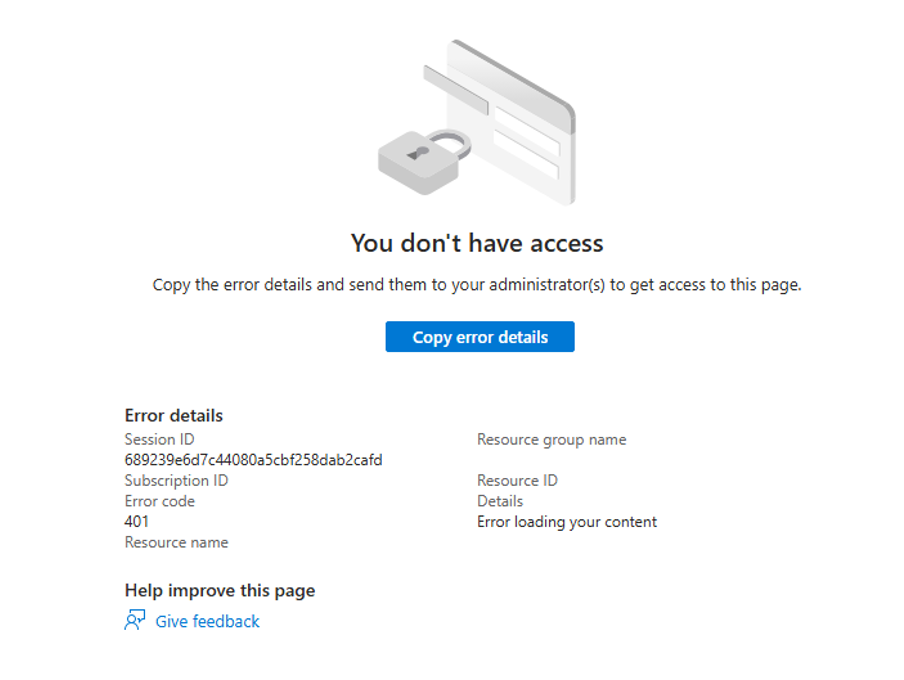
\includegraphics[width=0.7\linewidth]{figures/perm.png}
    \caption{Erro \texttt{401 (Unauthorized)} no portal do Azure ao tentar
        registar a aplicação no \emph{tenant} da UAlg.}\label{fig:azure401}
\end{figure}

\paragraph{Justificação da solução implementada.}

\begin{itemize}[leftmargin=*]
    \item \textbf{Independência de infraestrutura:} o sistema funciona de forma
          autónoma, sem depender de autorizações de terceiros (Serviços de
          Informática) para operar.
    \item \textbf{Validação de domínio configurável:} o \emph{login} é
          intercetado pelo \emph{callback} \texttt{signIn} do NextAuth, que
          delega na função \texttt{isEmailAllowed} (\texttt{lib/auth-utils.ts})
          a verificação contra a variável de ambiente
          \texttt{ALLOWED\_EMAIL\_DOMAIN}.
    \item \textbf{Segurança:} mantém-se o princípio fundamental de não armazenar
          \emph{hashes} de \emph{passwords} na base de dados (a tabela
          \texttt{User} não possui campo \texttt{password}), mitigando o risco de
          fugas de dados. Os \emph{tokens} de \emph{magic link} expiram em
          5~minutos e só podem ser utilizados uma vez.
    \item \textbf{Experiência de utilizador (UX):} o fluxo de \emph{magic link}
          atua como um SSO simplificado --- o utilizador não precisa de
          memorizar uma nova \emph{password}, bastando clicar no link seguro
          enviado para a caixa de correio.
\end{itemize}

\paragraph{Nota sobre a restrição de domínio na demonstração.}
Embora o mecanismo de restrição esteja implementado e funcional, a sua
ativação em produção depende de que o domínio do remetente configurado no
Resend (utilizado para enviar os \emph{magic links}) seja aceite pelos
servidores de correio institucionais da UAlg. À data de submissão, o pedido
de \emph{whitelisting} do domínio remetente junto dos Serviços de Informática
da UAlg ainda não obteve resposta, pelo que os emails para destinatários
\texttt{@ualg.pt} não chegavam de forma fiável à caixa de entrada. Para
permitir a demonstração e a avaliação do projeto, a equipa optou por
desativar temporariamente a restrição de domínio (mantendo, ainda assim, o
código de validação intacto e ativável por configuração). Assim que o pedido
de \emph{whitelisting} for atendido, basta repor
\texttt{ALLOWED\_EMAIL\_DOMAIN=ualg.pt} no Railway --- sem qualquer alteração
de código --- para que a restrição volte a aplicar-se.

\subsubsection{4. Modelação de Dados e Resolução de Conflitos}

Durante a modelação, surgiram desafios de nomenclatura e de \emph{design} que
foram resolvidos através de uma separação clara de conceitos no
\texttt{schema.prisma}:

\begin{itemize}[leftmargin=*]
    \item \textbf{\emph{Auth} vs. negócio:}
          \begin{itemize}
              \item \texttt{Session} (\emph{Auth}) -- mantida estritamente para a
                    gestão de sessões de \emph{login} (\emph{cookies}) do NextAuth.
              \item \texttt{StudySession} (negócio) -- criada para representar as
                    sessões de estudo ou reservas de espaços. Esta distinção evita
                    conflitos no código e clarifica o propósito de cada tabela.
          \end{itemize}
    \item \textbf{Identificação do estudante:} adicionou-se o campo
          \texttt{studentId} ao modelo de utilizador para permitir a futura
          integração com cartões de estudante físicos ou sistemas académicos,
          separando o ID interno do sistema (CUID) do número de aluno.
    \item \textbf{Participação vs. pedido de adesão:} para modelar corretamente
          o ciclo de vida de um convite, foram introduzidas duas entidades
          distintas:
          \begin{itemize}
              \item \texttt{JoinRequest} -- representa um pedido de adesão a uma
                    sessão, com estado (\texttt{PENDING}, \texttt{ACCEPTED},
                    \texttt{REJECTED}).
              \item \texttt{UserOnStudySession} -- tabela-pivô com chave composta
                    \texttt{(userId, sessionId)} que regista a participação
                    \emph{efetiva} de um utilizador numa sessão, apenas depois de o
                    pedido ser aceite.
          \end{itemize}
    \item \textbf{Relações com flexibilidade futura:} estabeleceu-se uma relação
          $1{:}N$ entre \texttt{User} e \texttt{Account}, permitindo que um mesmo
          utilizador venha a associar múltiplos \emph{providers} de autenticação
          (e.g., se o SSO institucional se tornar viável no futuro).
\end{itemize}

\subsubsection{5. Infraestrutura: Docker}

O ambiente de desenvolvimento é padronizado via \textbf{Docker} (observável
pelos ficheiros \texttt{Dockerfile} e \texttt{compose.yaml}).

\begin{itemize}[leftmargin=*]
    \item \textbf{Justificação:} garante que todos os membros da equipa executam
          a mesma versão da base de dados PostgreSQL, eliminando erros do tipo
          ``funciona na minha máquina''. O arranque completo do ambiente faz-se
          com um único comando (\texttt{docker compose up}).
\end{itemize}

\subsubsection{6. Envio de Email: Migração de Nodemailer para Resend}\label{sec:resend}

O envio transacional de email (\emph{magic links} de autenticação, notificações
de pedidos de adesão a sessões, aprovações e rejeições) sofreu uma iteração
arquitetural relevante durante o desenvolvimento.

\paragraph{Implementação inicial: Nodemailer (SMTP).}
A primeira versão recorria ao \emph{adapter} \texttt{nodemailer} suportado pelo
\texttt{EmailProvider} do NextAuth, configurado para enviar via SMTP. Esta
abordagem é a \emph{default} sugerida pela documentação do NextAuth e exige
apenas credenciais SMTP (\emph{host}, porto, utilizador, \emph{password}).

\paragraph{Limitação encontrada: Resend não suporta SMTP no \emph{free tier}.}
Ao avançar para o \emph{deploy} em produção (ver \S5.4.7), a equipa avaliou
serviços de envio de email com \emph{free tier} adequado a um projeto académico.
O \textbf{Resend} foi o candidato natural pelo seu \emph{tier} gratuito
(3\,000 emails/mês) e API moderna. Contudo, ao contrário de provedores
clássicos (SendGrid, Mailgun, AWS SES), o \textbf{Resend não disponibiliza
\emph{endpoint} SMTP no \emph{free tier}} --- apenas a API HTTP nativa
(\texttt{POST /emails}). Esta limitação impossibilitou a reutilização direta do
\emph{adapter} \texttt{nodemailer} já integrado no NextAuth.

\paragraph{Solução adotada: cliente HTTP nativo do Resend.}
A integração foi refeita usando o SDK oficial \texttt{resend} (Node.js), que
encapsula chamadas à API HTTP. Em concreto:

\begin{itemize}[leftmargin=*]
    \item Foi criado o módulo \texttt{lib/send-notification-email.ts} que expõe
          funções tipadas (\texttt{sendJoinRequestEmail},
          \texttt{sendApprovedJoinRequestEmail},
          \texttt{sendNotAcceptedJoinRequestEmail},
          \texttt{sendVerificationRequestEmail}) sobre uma instância partilhada do
          cliente \texttt{Resend} (obtida via \emph{getter} para permitir
          injeção em testes).
    \item No \texttt{EmailProvider} do NextAuth, a \emph{callback}
          \texttt{sendVerificationRequest} foi substituída por uma implementação
          que invoca o cliente Resend diretamente, abandonando a chamada SMTP.
    \item As variáveis de ambiente foram reduzidas a \texttt{RESEND\_API\_KEY}
          e \texttt{EMAIL\_FROM}, simplificando a configuração no Railway face às
          múltiplas variáveis SMTP anteriores.
    \item Falhas no envio (\texttt{HTTP} $\neq$ 2xx) são capturadas e registadas
          sem bloquear o fluxo principal (e.g., a criação de um \texttt{JoinRequest}
          é persistida mesmo que a notificação por email falhe).
\end{itemize}

\paragraph{Justificação.} A migração, embora não planeada, foi vantajosa: a API
HTTP do Resend dispensa a manutenção de credenciais SMTP, oferece \emph{logs} e
métricas de entrega no \emph{dashboard} do próprio serviço e elimina problemas
recorrentes de \emph{firewall} / portos SMTP bloqueados em ambientes de
\emph{cloud}. O \emph{trade-off} foi o investimento na refatorização do
\emph{adapter} de email do NextAuth.

\subsubsection{7. Plataforma de \emph{Deploy}: Railway}\label{sec:railway}

A aplicação foi \emph{deployed} em ambiente de produção na plataforma
\textbf{Railway}, escolhida após análise de alternativas como Vercel, Render e
AWS Elastic Beanstalk.

\paragraph{Justificação.}
\begin{itemize}[leftmargin=*]
    \item \textbf{Suporte nativo a \emph{Dockerfile}:} a mesma imagem usada em
          desenvolvimento (\texttt{spot-on/Dockerfile}) é reutilizada em
          produção, garantindo paridade entre ambientes. Vercel, em contraste,
          obrigaria a abandonar Docker e a adaptar a aplicação ao seu
          \emph{runtime} \emph{serverless}.
    \item \textbf{PostgreSQL gerido no mesmo \emph{provider}:} a base de dados
          é provisionada com um clique e a \texttt{DATABASE\_URL} é injetada
          automaticamente como variável de ambiente, evitando a configuração
          manual de \emph{strings} de conexão entre serviços externos.
    \item \textbf{\emph{Deploy} contínuo a partir do GitHub:} cada \emph{push}
          em \texttt{main} desencadeia automaticamente uma \emph{build} e
          \emph{rollout}, alinhando-se com a \emph{pipeline} de CI já existente.
    \item \textbf{Configuração declarativa:} o ficheiro \texttt{railway.toml}
          declara explicitamente o comando de \emph{build} e o
          \texttt{preDeployCommand}, sendo versionado no repositório.
    \item \textbf{\emph{Free tier} adequado:} suficiente para o âmbito
          académico, sem necessidade de cartão de crédito.
\end{itemize}

\paragraph{Configuração específica.}
\begin{itemize}[leftmargin=*]
    \item \textbf{\texttt{spot-on/railway.toml}:} declara o ciclo de \emph{deploy}
          com apenas duas diretivas --- \texttt{preDeployCommand} (script de
          preparação da base de dados) e \texttt{startCommand}
          (\texttt{npm start}). A imagem é construída a partir do mesmo
          \texttt{Dockerfile} usado em desenvolvimento, garantindo paridade
          entre os ambientes.
    \item \textbf{Script \texttt{spot-on/scripts/predeploy.sh}:} encadeia
          \texttt{npx prisma db push --accept-data-loss --skip-generate}
          (sincronização do \emph{schema} contra a base de dados) e
          \texttt{npx tsx prisma/seed.ts} (\emph{seed} idempotente),
          garantindo que a base de dados arranca sempre num estado conhecido
          após cada \emph{rollout}.
    \item \textbf{Estratégia de \emph{schema}:} optou-se por
          \texttt{prisma db push} no \emph{predeploy} (em vez de
          \texttt{prisma migrate deploy}) por simplicidade durante a fase de
          desenvolvimento iterativo --- a \emph{flag}
          \texttt{--accept-data-loss} é tolerada porque o ambiente é
          re-\emph{seeded} a cada \emph{deploy}. O histórico de migrações em
          \texttt{prisma/migrations} continua a ser mantido para suportar a
          futura transição para \texttt{migrate deploy} num cenário de dados
          de produção persistentes.
    \item \textbf{Variáveis de ambiente em produção:}
          \texttt{DATABASE\_URL} (auto-injetada pelo Railway via \emph{service
              variables} do PostgreSQL gerido), \texttt{NEXTAUTH\_SECRET},
          \texttt{NEXTAUTH\_URL}, \texttt{QR\_SECRET},
          \texttt{ALLOWED\_EMAIL\_DOMAIN} (atualmente não definida, ver
          \S5.4.3), \texttt{LIBRARY\_CLOSING\_TIME},
          \texttt{RESEND\_API\_KEY} e \texttt{EMAIL\_FROM}.
\end{itemize}

\paragraph{Resumo.} Esta arquitetura privilegia a \textbf{segurança} (ao
remover \emph{passwords} e validar o domínio institucional), a
\textbf{integridade} (via PostgreSQL + Prisma com migrações versionadas) e a
\textbf{manutenibilidade} (TypeScript + Next.js com tipagem partilhada),
criando uma base sólida para o desenvolvimento das funcionalidades de gestão
de espaços da UAlg.

% =====================================================
% 6. Modelo de Dados
% =====================================================
\section{Modelo de Dados}\label{sec:data}

A persistência é definida no \emph{schema} Prisma
(\texttt{spot-on/prisma/schema.prisma}). As entidades dividem-se em dois
grupos: as relativas à autenticação (\texttt{User}, \texttt{Account},
\texttt{Session}, \texttt{VerificationToken}, herdadas do modelo do
NextAuth.js) e as do domínio Spot-On.

\subsection{Entidades de Domínio}

\begin{table}[H]
    \centering
    \renewcommand{\arraystretch}{1.3}
    \begin{tabularx}{\linewidth}{@{}lX@{}}
        \toprule
        \textbf{Entidade}           & \textbf{Descrição}                                                                                                                                                        \\
        \midrule
        \texttt{User}               & Utilizador autenticado. Inclui \texttt{studentId} opcional, pontos acumulados (\texttt{points}) e prazo de banimento (\texttt{bannedUntil}), se aplicável.                \\
        \texttt{FloorPlan}          & Planta de um piso da biblioteca; serve de \emph{canvas} sobre o qual os espaços são posicionados.                                                                         \\
        \texttt{Space}              & Espaço de estudo (mesa individual ou sala de grupo). Inclui geometria (\emph{points} SVG), capacidade, atributos (tomada, computador, quadro interativo) e o QR rotativo. \\
        \texttt{StudySession}       & Sessão de estudo num espaço, com anfitrião, hora prevista de fim e estado (\texttt{ACTIVE}, \texttt{COMPLETED}, \texttt{EXPIRED}).                                        \\
        \texttt{JoinRequest}        & Pedido de adesão de um utilizador a uma sessão de estudo, com estado (\texttt{PENDING}, \texttt{ACCEPTED}, \texttt{REJECTED}).                                            \\
        \texttt{UserOnStudySession} & Tabela-pivô que regista a participação efetiva de um utilizador numa sessão (após aceitação do pedido), com \emph{timestamp} de adesão.                                   \\
        \texttt{Report}             & \emph{Report} submetido por um utilizador sobre uma sessão, com janela de confirmação de 10 minutos.                                                                      \\
        \texttt{ReportConfirmation} & Confirmação de um \emph{report} por um terceiro utilizador.                                                                                                               \\
        \texttt{Notification}       & Notificação \emph{in-app} dirigida a um utilizador (e.g., pedido de adesão, prova de presença, sessão a expirar).                                                         \\
        \texttt{Badge}              & Insígnia que pode ser atribuída (mensal, anual ou permanente).                                                                                                            \\
        \texttt{UserBadge}          & Tabela-pivô que regista a atribuição de \emph{badges} a utilizadores.                                                                                                     \\
        \bottomrule
    \end{tabularx}
    \caption{Entidades do modelo de domínio Spot-On.}
\end{table}

O modelo recorre ainda a vários \emph{enum types} nativos do PostgreSQL:
\texttt{SessionStatus}, \texttt{JoinRequestStatus}, \texttt{SpaceType},
\texttt{SpaceShape}, \texttt{ReportStatus}, \texttt{NotificationType} e
\texttt{NotificationStatus}.

\subsection{Diagrama do Modelo de Dados}

A Figura~\ref{fig:classdiag} apresenta o diagrama UML de classes do modelo de
domínio, mantido em formato \emph{drawio} no repositório
(\texttt{diagrams/class/domain\_class\_diagram.drawio}) e exportado como PNG
para inclusão neste relatório. A análise detalhada das relações e das
escolhas de modelação é apresentada na subsecção seguinte.

\begin{figure}[H]
    \centering
    % Substituir pelo PNG exportado do drawio quando estiver finalizado:
    % \includegraphics[width=0.95\linewidth]{figures/class_diagram.png}
    \vspace{1em}\textit{[Diagrama a inserir: \texttt{figures/class\_diagram.png}]}\vspace{1em}
    \caption{Diagrama UML de classes do modelo de domínio.}\label{fig:classdiag}
\end{figure}

\subsection{Decisões de Modelação Relevantes}

\begin{itemize}[leftmargin=*]
    \item \textbf{Geometria dos espaços armazenada como \emph{string} SVG.}
          O atributo \texttt{points} de \texttt{Space} segue o formato
          \texttt{"x1,y1 x2,y2 \dots"}, compatível com o elemento \texttt{<polygon>}
          do SVG. Esta decisão evita a sobrecarga de uma tabela auxiliar de vértices
          e permite \emph{rendering} direto na interface.
    \item \textbf{Token QR rotativo.} O atributo \texttt{currentQrToken} é
          único e atualizado periodicamente por uma rotina do servidor (\emph{cron
              job} com \texttt{node-cron}), impedindo que um QR fotografado uma única
          vez possa ser reutilizado posteriormente.
    \item \textbf{Janela de confirmação de \emph{reports}.} O campo
          \texttt{timeToConfirm} usa o valor por omissão gerado na base de dados
          (\texttt{now() + interval '10 minutes'}), garantindo coerência mesmo
          perante dessincronização horária no \emph{frontend}.
    \item \textbf{Separação \texttt{JoinRequest} / \texttt{UserOnStudySession}.}
          O ciclo de vida de um convite é modelado em duas tabelas distintas: a
          primeira regista a intenção de participar (com estado evolutivo), a
          segunda regista apenas a participação confirmada. Esta separação evita
          ambiguidade sobre o estado atual e simplifica as consultas.
    \item \textbf{Tabelas-pivô explícitas com chave composta.}
          \texttt{UserOnStudySession}, \texttt{ReportConfirmation} e
          \texttt{UserBadge} são modeladas como entidades próprias por carregarem
          informação adicional (\texttt{joinedAt}, \texttt{confirmedAt},
          \texttt{awardedAt}).
    \item \textbf{Banimento como \texttt{DateTime}.}
          \texttt{User.bannedUntil} guarda diretamente o instante até ao qual o
          banimento é válido, eliminando a necessidade de um \emph{flag} associado a
          uma data calculada.
\end{itemize}

\subsection{Excerto do \emph{Schema} Prisma}

A título ilustrativo, apresenta-se a definição da entidade central
\texttt{Space}:

\begin{lstlisting}[language=Java]
model Space {
  id                  String      @id @default(cuid()) @db.VarChar(30)
  floorPlanId         String      @db.VarChar(30)
  name                String      @db.VarChar(255)
  points              String      /// pontos SVG do polígono
  capacity            Int
  currentQrToken      String      @unique @db.VarChar(255)
  description         String?     @db.VarChar(255)
  hasPowerOutlet      Boolean     @default(false)
  hasComputer         Boolean     @default(false)
  hasInteractiveBoard Boolean     @default(false)
  type                SpaceType   @default(INDIVIDUAL_DESK)
  shape               SpaceShape?

  createdAt DateTime @default(now())
  updatedAt DateTime @default(now()) @updatedAt

  floorPlan    FloorPlan      @relation(fields: [floorPlanId], references: [id], onDelete: Cascade)
  sessions     StudySession[]
  joinRequests JoinRequest[]
}
\end{lstlisting}

% =====================================================
% 8. Backend e API
% =====================================================
\section{Backend e API}\label{sec:backend}

O \emph{backend} é exposto como uma \textbf{API REST de serviços}, suportada
pelas \emph{API routes} do Next.js sob \texttt{/api/*}. Cada \emph{endpoint}
é documentado de forma interativa através de \textbf{Swagger / OpenAPI},
servida pela aplicação em \texttt{/api-doc} (componente
\texttt{ReactSwagger}, baseado em \texttt{next-swagger-doc} e
\texttt{swagger-ui-react}). A especificação é gerada automaticamente a
partir de anotações JSDoc \texttt{@swagger} colocadas em cada rota,
mantendo a documentação sincronizada com o código. Os grupos de
\emph{endpoints} atualmente disponíveis são:

\begin{itemize}[leftmargin=*]
    \item \texttt{/api/auth/*} -- \emph{endpoints} geridos pelo NextAuth.js
          (envio de \emph{magic links}, \emph{callbacks}, \emph{sign-out}).
    \item \texttt{/api/spaces/*} -- gestão e consulta de espaços, plantas e
          sessões de estudo associadas (incluindo criação, adesão, prolongamento,
          \emph{check-out} e \emph{reports}).
    \item \texttt{/api/qrcode/*} -- emissão e validação dos \emph{tokens} QR
          rotativos dos espaços.
    \item \texttt{/api/notifications/*} -- consulta e atualização de
          notificações \emph{in-app}.
    \item \texttt{/api/leaderboard} -- exposição dos rankings de pontuação para
          a componente de gamificação.
    \item \texttt{/api/user/*} -- consulta e atualização do perfil do
          utilizador autenticado.
\end{itemize}

Cada \emph{endpoint} obtém a sessão via \texttt{getServerSession}, valida os
dados de entrada e delega o acesso a dados ao Prisma \emph{Client}. A proteção
de rotas de UI é complementada por um \emph{middleware} (\texttt{proxy.ts})
que valida a presença do \emph{cookie} de sessão antes de servir páginas
privadas.

A persistência é orientada pelo \emph{schema} declarativo
\texttt{prisma/schema.prisma}. Em desenvolvimento, cada alteração do
\emph{schema} gera uma nova migração SQL via
\texttt{npx prisma migrate dev}, ficando registada no diretório
\texttt{prisma/migrations} (à data, 14 migrações cobrindo desde a criação
inicial do \emph{schema} até à introdução do modelo \texttt{JoinRequest},
do campo \texttt{bannedUntil} e dos tipos de notificação). Em produção, o
\emph{predeploy} no Railway sincroniza o \emph{schema} contra a base de dados
via \texttt{prisma db push}, conforme descrito em \S5.4.7.

% =====================================================
% 9. Controlo de Versões
% =====================================================
\section{Controlo de Versões}

Todo o desenvolvimento é gerido em Git, com repositório alojado no GitHub e
partilhado em modo de leitura com os docentes. Cada elemento da equipa
contribui sob a sua identidade pessoal, garantindo que o histórico reflete
fielmente a contribuição individual.

\paragraph{Fluxo adotado.}
Foi seguido um modelo simplificado baseado em \emph{feature branches}:

\begin{enumerate}[leftmargin=*]
    \item Cada \emph{user story} ou tarefa origina um \emph{branch} dedicado
          (\texttt{feature/<descrição>});
    \item A integração no \emph{branch} principal (\texttt{main}) ocorre
          exclusivamente via \emph{pull request};
    \item Cada \emph{pull request} requer revisão por outro elemento da
          equipa antes de \emph{merge};
    \item A \emph{pipeline} de CI deve passar (\emph{lint}, testes,
          \emph{build}) como pré-condição.
\end{enumerate}

% =====================================================
% 10. Gestão de Projeto (SCRUM)
% =====================================================
\section{Gestão de Projeto -- SCRUM}

A gestão do projeto seguiu a metodologia SCRUM, suportada pela plataforma
Jira. Definiu-se um \emph{product backlog} composto por \emph{user stories}
com critérios de aceitação claros. As \emph{stories} foram refinadas e
priorizadas no início de cada \emph{sprint}.

\paragraph{Cerimónias.}
Cada \emph{sprint} (com duração de \textbf{duas} semanas) inclui:
\begin{itemize}[leftmargin=*]
    \item \textbf{\emph{Sprint planning}} -- seleção das \emph{stories} a
          incluir no \emph{sprint};
    \item \textbf{\emph{Daily}} -- ponto de situação curto entre os elementos;
    \item \textbf{\emph{Sprint review}} -- demonstração do incremento;
    \item \textbf{\emph{Retrospetiva}} -- análise do que correu bem, do que
          deve melhorar e ações a tomar.
\end{itemize}

\paragraph{Evidências.} O Jira mantém o histórico de \emph{sprints}, cartões
movidos entre estados (\emph{To Do}, \emph{In Progress}, \emph{In Review},
\emph{Done}), e os \emph{burndown charts} associados.

% =====================================================
% 11. Testes e Integração Contínua
% =====================================================
\section{Testes e Integração Contínua}

\subsection{Testes Automatizados}

A estratégia de testes combina \textbf{Jest} (executado quer localmente quer
na \emph{pipeline} de CI) com uma \emph{suite} \textbf{Postman/Newman}
adicional para validação \emph{end-to-end} da API. O código de teste está
organizado da seguinte forma:

\begin{itemize}[leftmargin=*]
    \item \textbf{Testes unitários} (\texttt{spot-on/\_\_tests\_\_/unit/}) --
          cobrem funções isoladas de lógica de negócio, e.g., utilitários de
          autenticação (\texttt{auth-utils.test.ts}), geração e validação dos
          \emph{tokens} QR dinâmicos (\texttt{dynamic-qrcode.test.ts}), regras de
          expiração de \emph{reports} (\texttt{ReportExpiry.test.ts}) e
          notificações.
    \item \textbf{Testes de integração}
          (\texttt{spot-on/\_\_tests\_\_/integration/}) -- exercitam os
          \emph{endpoints} da API contra uma instância real de PostgreSQL e um
          servidor Next.js em execução. Cobrem os fluxos críticos: sessões de
          estudo (criação, adesão, prolongamento, libertação, expiração),
          \emph{reports} ativos, QR code, leaderboard, espaços e \emph{badges}.
    \item \textbf{Testes \emph{end-to-end} da API}
          (\texttt{spot-on/postman/}) -- coleção Postman executável via Newman,
          com \emph{seed} dedicado (\texttt{seed-test.ts}) que prepara o estado da
          base de dados antes da execução.
\end{itemize}

\subsection{Pipeline de CI}

A \emph{pipeline} é definida em \texttt{.github/workflows/ci.yml} e dispara
em cada \emph{push} para \texttt{main}, \texttt{develop} ou \emph{branches}
\texttt{feature/**}/\texttt{fix/**}, bem como em cada \emph{pull request} para
\texttt{main} ou \texttt{develop}. Estão definidos três \emph{jobs}
encadeados:

\begin{enumerate}[leftmargin=*]
    \item \textbf{Lint} -- análise estática com ESLint (\texttt{npm run lint}).
    \item \textbf{Test} -- arranca um serviço PostgreSQL 17, gera o cliente
          Prisma (\texttt{npx prisma generate}), levanta um servidor Next.js de
          teste em \texttt{localhost:3001} e executa a \emph{suite} Jest unitária
          e de integração (\texttt{npm test}).
    \item \textbf{Build} -- depende de \emph{lint} e \emph{test}, instala
          dependências e executa \texttt{npm run build} (\texttt{next build}) para
          garantir que a aplicação compila para produção sem erros.
\end{enumerate}

Adicionalmente, o workflow \texttt{codeql.yml} executa análise de segurança
estática (\emph{CodeQL}) sobre o código TypeScript. A passagem de todos os
\emph{jobs} é pré-condição obrigatória para a aprovação dos \emph{pull
    requests}.

% =====================================================
% 12. Deployment
% =====================================================
\section{Deployment}

\subsection{Execução Local}\label{sec:local}

A execução local da aplicação assenta em \textbf{Docker Compose}, com dois
serviços declarados em \texttt{spot-on/compose.yaml}: o serviço \texttt{web}
(aplicação Next.js, construída a partir de \texttt{spot-on/Dockerfile}) e o
serviço \texttt{db} (instância de PostgreSQL 17). Importa sublinhar que o
\textbf{mesmo \texttt{Dockerfile}} é reutilizado em produção pelo Railway
(ver \S\ref{sec:railway} e \S\ref{sec:prod}), garantindo paridade total
entre os dois ambientes.

\paragraph{Pré-requisitos.}
\begin{itemize}[leftmargin=*]
    \item \textbf{Git} -- para clonar o repositório.
    \item \textbf{Docker} e \textbf{Docker Compose} -- únicos requisitos
          obrigatórios para o fluxo recomendado.
    \item \textbf{GNU Make} (recomendado) -- simplifica o arranque para um
          único comando; opcional, todas as operações podem ser invocadas
          diretamente via \texttt{docker compose}.
    \item \textbf{Node.js 20+} e \texttt{npm} -- apenas necessários para o
          fluxo alternativo de execução do Next.js diretamente no \emph{host}.
\end{itemize}

\paragraph{Variáveis de ambiente.}
O repositório inclui um ficheiro \texttt{spot-on/.env} com valores
\emph{default} sensatos para desenvolvimento local, pelo que o \emph{stack}
arranca sem necessidade de configuração adicional. As variáveis principais
estão descritas em detalhe em \S\ref{sec:prod}; a única que pode requerer
ajuste é \texttt{NEXTAUTH\_URL}, que tem de corresponder ao endereço real do
\emph{host} (\texttt{localhost} para uso na própria máquina ou IP da LAN
para teste em telemóvel via QR code).

\paragraph{Opção A --- \emph{Makefile} (recomendada).}
O ficheiro \texttt{spot-on/Makefile} encapsula as operações comuns em
\emph{targets} nomeados. O arranque completo do \emph{stack} faz-se com:

\begin{lstlisting}[language=bash]
make docker-recreate
\end{lstlisting}

Este \emph{target} executa, em sequência: \texttt{docker compose down -v}
$\to$ \texttt{build --no-cache} $\to$ \texttt{up -d} $\to$ aguarda que o
\emph{container} \texttt{web} responda $\to$ executa \texttt{prisma generate}
e \texttt{prisma db seed} $\to$ segue os \emph{logs}. No final, a aplicação
está acessível em \href{http://localhost:3000}{\texttt{http://localhost:3000}}.

\noindent Outros \emph{targets} úteis no dia-a-dia:

\begin{itemize}[leftmargin=*]
    \item \texttt{make docker-up} / \texttt{make docker-down} --- iniciar /
          parar o \emph{stack} (com remoção de volumes).
    \item \texttt{make docker-logs} --- seguir os \emph{logs} dos
          \emph{containers}.
    \item \texttt{make docker-seed} --- re-executar o \emph{seed} dentro do
          \emph{container} \texttt{web} em execução.
    \item \texttt{make test} / \texttt{make test-watch} --- executar a
          \emph{suite} Jest (uma vez ou em \emph{watch mode}).
    \item \texttt{make lint} / \texttt{make lint-fix} --- análise estática
          ESLint (leitura ou auto-correção).
    \item \texttt{make prisma-studio} --- abrir Prisma Studio (\emph{browser}
          visual da base de dados em \texttt{http://localhost:5555}).
    \item \texttt{make swagger-open} --- abrir a documentação Swagger UI no
          \emph{browser} (\texttt{/api-doc}).
    \item \texttt{make postman-ci} --- correr a \emph{suite}
          \emph{end-to-end} Newman contra uma base de dados de teste
          isolada.
\end{itemize}

\paragraph{Opção B --- Docker Compose (manual).}
Equivalente direto da Opção A, sem o \emph{wrapper} do \emph{Makefile}.
Reconstrução completa:

\begin{lstlisting}[language=bash]
docker compose down -v
docker compose build --no-cache
docker compose up -d
docker compose logs -f web
\end{lstlisting}

O \emph{entrypoint} do \emph{container} \texttt{web} executa automaticamente
\texttt{prisma generate}, aguarda a base de dados, aplica
\texttt{prisma db push}, executa o \emph{seed} e inicia \texttt{next dev} ---
não há passos manuais adicionais.

\paragraph{Opção C --- Node.js no \emph{host} (alternativa).}
Útil para iterações rápidas em macOS/Windows (\emph{file-watching} mais
eficiente que dentro do \emph{container}). Apenas a base de dados é
containerizada:

\begin{lstlisting}[language=bash]
npm install                     # inclui prisma generate via postinstall
docker compose up -d db         # apenas o serviço Postgres
npx prisma migrate dev          # aplica migrações
npx prisma db seed              # popula a base de dados
npm run dev                     # inicia o servidor de desenvolvimento
\end{lstlisting}

Em qualquer das opções, o \emph{seed} popula a base de dados com plantas dos
pisos, espaços, utilizadores de demonstração, sessões ativas e
\emph{reports}, permitindo experimentar imediatamente as funcionalidades sem
necessidade de criar dados manualmente.

\subsection{Ambiente de Produção (Railway)}\label{sec:prod}

O ambiente de produção corre na plataforma \textbf{Railway}, escolhida pelas
razões detalhadas em \S\ref{sec:railway}. O \emph{deploy} é contínuo a partir
do \emph{branch} \texttt{main} do repositório GitHub: cada \emph{push}
desencadeia automaticamente uma nova \emph{build}, a aplicação das migrações
da base de dados e o arranque da nova versão da aplicação. O mesmo
\texttt{Dockerfile} utilizado em desenvolvimento serve de base para a imagem
de produção, garantindo paridade entre ambientes.

\paragraph{Configuração declarativa (\texttt{railway.toml}).}
A configuração do \emph{deploy} está versionada no repositório através do
ficheiro \texttt{spot-on/railway.toml}, com apenas duas diretivas:

\begin{lstlisting}[language=bash]
[deploy]
preDeployCommand = "sh scripts/predeploy.sh"
startCommand     = "npm start"
\end{lstlisting}

A imagem da aplicação é construída automaticamente pelo Railway a partir do
mesmo \texttt{Dockerfile} usado no \emph{compose} local. O script
\texttt{scripts/predeploy.sh} é executado antes do arranque de cada
\emph{rollout}:

\begin{lstlisting}[language=bash]
#!/bin/sh
set -e
echo "==> [predeploy] Pushing Prisma schema"
npx prisma db push --accept-data-loss --skip-generate
echo "==> [predeploy] Running seed"
npx tsx prisma/seed.ts
\end{lstlisting}

\paragraph{Variáveis de ambiente em produção.}
A gestão de \emph{secrets} é feita no painel do Railway. As variáveis
configuradas são:

\begin{itemize}[leftmargin=*]
    \item \texttt{DATABASE\_URL} -- injetada automaticamente pelo serviço
          PostgreSQL gerido do Railway via \emph{service variables}.
    \item \texttt{NEXTAUTH\_SECRET} e \texttt{NEXTAUTH\_URL} -- usadas pelo
          NextAuth para assinar e validar as sessões.
    \item \texttt{QR\_SECRET} -- chave HMAC para assinatura dos \emph{tokens}
          QR dinâmicos.
    \item \texttt{ALLOWED\_EMAIL\_DOMAIN} -- restrição opcional do domínio de
          email (atualmente não definida, ver \S\ref{sec:resend} e \S5.4.3).
    \item \texttt{LIBRARY\_CLOSING\_TIME} -- hora de fecho da biblioteca
          (UTC, formato \texttt{HH:MM}), usada para limitar o
          \texttt{expectedEndTime} das sessões.
    \item \texttt{RESEND\_API\_KEY} e \texttt{EMAIL\_FROM} -- credenciais e
          remetente para o envio de email via Resend (ver \S\ref{sec:resend}).
\end{itemize}

\paragraph{Provisioning da base de dados.}
O PostgreSQL é provisionado como serviço independente no mesmo projeto
Railway. A \texttt{DATABASE\_URL} é partilhada entre serviços através do
mecanismo de \emph{service variables} do Railway, sem necessidade de copiar
a \emph{connection string} manualmente.

% =====================================================
% 13. Conformidade com o Enunciado
% =====================================================
\section{Conformidade com o Enunciado}

A tabela seguinte mapeia, de forma direta, cada requisito formal do enunciado
do trabalho prático à secção (ou ficheiro) onde a evidência pode ser
encontrada.

\begin{table}[H]
    \centering
    \footnotesize
    \renewcommand{\arraystretch}{1.3}
    \begin{tabularx}{\linewidth}{@{}p{4.2cm}Xc@{}}
        \toprule
        \textbf{Requisito do enunciado}                         & \textbf{Evidência no projeto / relatório}                                                                              & \textbf{Onde}                          \\
        \midrule
        \emph{Stack tecnológica} de escolha livre               & Next.js + TypeScript + Prisma + PostgreSQL + NextAuth + Resend + Docker + Railway.                                     & \S\ref{sec:arch}, Tab.~\ref{tab:stack} \\
        Justificação com pelo menos uma alternativa por camada  & Tabela ``Sumário da Stack e Alternativas'' (Tab.~\ref{tab:stack}) e \S5.4 (7 decisões com alternativas).               & \S\ref{sec:arch}, Tab.~\ref{tab:stack} \\
        \emph{Backend} separado, sob a forma de API documentada & API REST sob \texttt{/api/*}; documentação Swagger/OpenAPI em \texttt{/api-doc} gerada de anotações \texttt{@swagger}. & \S\ref{sec:backend}                    \\
        Persistência de dados obrigatória                       & Base de dados PostgreSQL 17.                                                                                           & \S\ref{sec:data}                       \\
        Utilização de um ORM                                    & Prisma com \emph{schema} declarativo e cliente tipado.                                                                 & \S5.4.2, \S\ref{sec:data}              \\
        Versionamento / migrações da base de dados              & 14 migrações em \texttt{prisma/migrations/} geradas via \texttt{prisma migrate dev} em desenvolvimento; sincronização do \emph{schema} em produção via \texttt{prisma db push}. & \S\ref{sec:backend}, \S5.4.7      \\
        Visão geral do sistema                                  & Descrição funcional, atores, requisitos.                                                                               & \S\ref{sec:overview}--\ref{sec:req}    \\
        Diagrama de arquitetura de alto nível                   & Diagrama de componentes (Figura~\ref{fig:arch}).                                                                       & \S5.1                                  \\
        Modelo de dados                                         & Entidades, enums, diagrama (Figura~\ref{fig:classdiag}) e excerto do \emph{schema}.                                    & \S\ref{sec:data}                       \\
        Justificação das decisões técnicas e arquiteturais      & 7 decisões numeradas com justificação e alternativas; iterações SSO~$\to$~Magic Links e Nodemailer~$\to$~Resend documentadas. & \S5.4                            \\
        \emph{Deployment} em produção                           & Plataforma Railway com \texttt{railway.toml}, \texttt{predeploy.sh} e PostgreSQL gerido.                               & \S5.4.7, \S11.2                        \\
        \bottomrule
    \end{tabularx}
    \caption{Mapa de conformidade entre os requisitos do enunciado e as
        secções deste relatório.}
\end{table}

% =====================================================
% 14. Conclusão
% =====================================================
\section{Conclusão}

O Spot-On materializa uma solução completa para um problema concreto vivido
diariamente na biblioteca da Universidade do Algarve. Do ponto de vista de
engenharia de software, o projeto permitiu aplicar boas práticas em todas as
fases: levantamento e priorização de requisitos sob SCRUM, desenho de uma
arquitetura clara e justificada, implementação com tecnologias modernas e
tipadas, persistência versionada com migrações, testes automatizados,
\emph{deployment} reprodutível e Integração Contínua.

Como trabalho futuro, identificam-se eixos como (i) a integração com sistemas
de \emph{notification push} para alertas em tempo real, (ii) a exposição de
estatísticas agregadas de utilização para apoio à gestão da biblioteca e (iii)
o alargamento do sistema a outros campi da Universidade.

\end{document}
